%!TEX root = ../main.tex

\chapter{GraphDB}
\chapterauthor{Thore Krüss, Lennart Purucker, Johanna Sommer}

\section{Motivation/Introduction}
First paragraph to state the general context and make important points for the motivation and why its important. Refer to Wood Paper here.

But Graph Database research has its beginnings already in the early 90s. During this time, numerous proposals came up, describing a semantic network to store data about the database. That was, because contemporary systems were failing to take into account the semantics of a database. (letzten Satz ändern)
The Locial Data Model \cite{KUPERLDM} was proposed, trying to combine the advantages of relational, hierarchical and network approaches in that they modeled databases as directed graphs, with leaves representing attributes and internal nodes posing as connections between the data. \\
Similar to that, the Functional Data Model \cite{Shipman1979} was proposed with the same goal, focusing specifically on providing a conceptually natural database interface \cite{Angles2018AnIT}. \\
During this period, most of the underlying theory of Graph Databases was created.
It was most likely because of insufficient hardware support for big graphs that this research declined, only to be picked up again now, powered by improved hardware. Todays focus in Graph Theory research lies primarily on actual practical systems and on the theoretical analysis of graph query languages \cite{Angles2018AnIT}.

Especially practical implementations of Graph Database Theory have gained traction, as real world problems are more often than not interrelated - hence graphs are extremely useful in unterstanding the wide diversity of real-world datasets.\cite{Robinson2013} \\
The emerging of social networks have naturally helped graph database models come up, with big players like Twitter and their implementation FlockDB entering the field. In those social network situations, a so-called social graph can effortlessly model attributes of a person as well as relationships between people. While in traditional RDBMS the apparent friend-of-a-friend-problem would be solved with a join over all relevant tables, in graph database technology this can be achieved with a traversal, which is far more cost inexpensive (letzten Teilsatz ändern) \cite{Miller2013GraphDA}. \\
Another meaningful topic today are recommender systems, where most work focusing on optimizing machine learning algorithms. But also in database theory, this specific context poses challenges. However again, the graph model gracefully maps item similarities and correlations between user behaviour \cite{Huang2002}.

These application fields bring very distinct workloads that require specific query languages to process. There are two different kinds of workload: in social network transactions low-latency online graphs are processed while for example link analysis algorithms evaluate high-throughput offline graphs \cite{Angles2018AnIT}. Many query language proposals have come up recently, differing mainly in the underlying graph data structure/model and the functionality provided \cite{Wood2012QueryLF}.

A deeper description of the theory behind graph databases will be given in subsection 2, aiming to connect the data model to its fields of application as well as comparing it to RDBMS. This comparison will be picked up in subsection 3, where a use case from the SQL world will be applied to Graph Database Theory, focusing in particular on Neo4j. Lastly, our findings will be stated in subsection 4 with a general conclusion.


\section{Graph Database Theory}
\subsection{Description of data model and functionality}
\subsection{fields of application}
\subsection{CAP Theorem}
\subsection{GraphDB vs. RDBMS}

\section{Implementation with Neo4j}
In this section the general setup of Neo4j should be lined out and a sample project be described utilizing available Python-Libraries to implement a sample use case.
\subsection{Use Case from the SQL world}
\subsection{Installation}
\subsection{Modelling}
The database model has been implemented using neomodel, which is a community driven project to provide an Object-Graph-Mapper (OGM) published under MIT-License.
The database model in \ref{lst:graphdb:neomodel} has been built following the neomodel documentation \cite{neomodel:rtd} describing a simple database structure.
This database maps the relations in a social network.
There may be an arbitrary number of Persons who may be friends with other persons.
Additionally they can state interests and may be a member of a group.
Forthermore they can state where they live (region and country).

\begin{figure}[h]
    \centering
    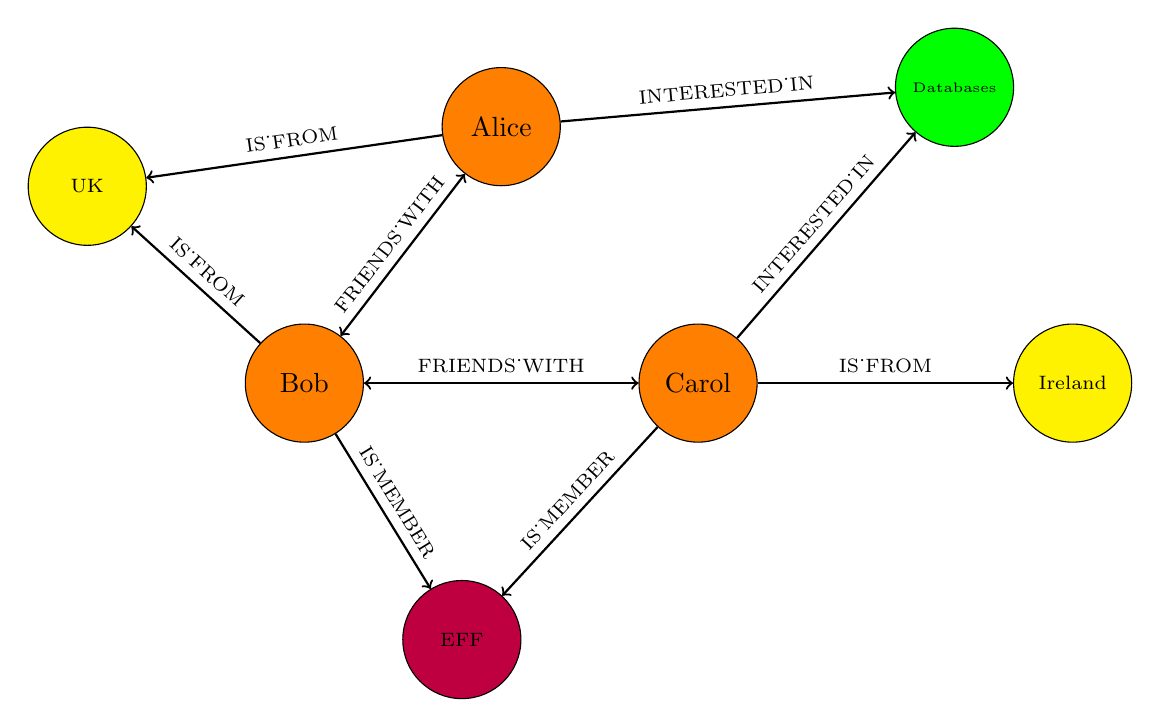
\begin{tikzpicture}
        \node[draw, circle, fill=orange, minimum height=1.5cm, minimum width=1.5cm] (alice) {Alice};
        \node[draw, circle, fill=orange, minimum height=1.5cm, minimum width=1.5cm] (bob)  at ([xshift=-2.5cm, yshift=-2.5cm]alice.south) {Bob};
        \node[draw, circle, fill=orange, minimum height=1.5cm, minimum width=1.5cm] (carol)  at ([xshift=2.5cm, yshift=-2.5cm]alice.south) {Carol};

        \node[draw, circle, fill=green, minimum height=1.5cm, minimum width=1.5cm] (db) at ([xshift=5cm, yshift=0.5cm]alice.east) {\tiny Databases};

        \node[draw, circle, fill=purple, minimum height=1.5cm, minimum width=1.5cm, align=center] (python) at ([xshift=2cm, yshift=-2.5cm]bob.south) {\scriptsize EFF};

        \node[draw, circle, fill=yellow, minimum height=1.5cm, minimum width=1.5cm] (uk) at ([xshift=-2cm, yshift=2.5cm]bob.west) {\scriptsize UK};
        \node[draw, circle, fill=yellow, minimum height=1.5cm, minimum width=1.5cm] (ire) at ([xshift=4cm]carol.east) {\scriptsize Ireland};



        \draw [<->, thick] (alice) -- (bob) node[midway,sloped, above] {{\scriptsize FRIENDS\char`_WITH}};

        \draw [<->, thick] (bob) -- (carol) node[midway,sloped, above] {\scriptsize FRIENDS\char`_WITH};

        \draw [->, thick] (alice) -- (db) node[midway,sloped, above] {\scriptsize INTERESTED\char`_IN};
        \draw [->, thick] (carol) -- (db) node[midway,sloped, above] {\scriptsize INTERESTED\char`_IN};

        \draw [->, thick] (bob) -- (python) node[midway,sloped, above] {\scriptsize IS\char`_MEMBER};
        \draw [->, thick] (carol) -- (python) node[midway,sloped, above] {\scriptsize IS\char`_MEMBER};

        \draw [->, thick] (alice) -- (uk) node[midway,sloped, above] {{\scriptsize IS\char`_FROM}};
        \draw [->, thick] (carol) -- (ire) node[midway,sloped, above] {{\scriptsize IS\char`_FROM}};
        \draw [->, thick] (bob) -- (uk) node[midway,sloped, above] {{\scriptsize IS\char`_FROM}};

    \end{tikzpicture}
    \caption{Sample database schema}
    \label{fig:graphdb:graphmodel}
\end{figure}


\begin{listing}[ht]
\begin{minted}{python}
from datetime import datetime

import pytz
from neomodel import (BooleanProperty, DateTimeProperty, IntegerProperty,
                      Relationship, RelationshipFrom, RelationshipTo,
                      StringProperty, StructuredNode, StructuredRel,
                      UniqueIdProperty, config)

class Partnership(StructuredRel):
    relationshipType = StringProperty()
    since = DateTimeProperty(
        default=lambda: datetime.now(pytz.utc)
    )

class Country(StructuredNode):
    name = StringProperty(unique_index=True, required=True)

class Region(StructuredNode):
    name = StringProperty(unique_index=True, required=True)

class Interest(StructuredNode):
    name = StringProperty(unique_index=True, required=True)

class Group(StructuredNode):
    name = StringProperty(unique_index=True, required=True)

class Person(StructuredNode):
    uid = UniqueIdProperty()
    name = StringProperty(unique_index=True)
    age = IntegerProperty(index=True, default=0)
    url = StringProperty()

    # traverse outgoing relations
    country = RelationshipTo(Country, 'IS_FROM')
    region = RelationshipTo(Region, 'IS_FROM')
    interests = RelationshipTo(Interest, 'IS_INTERESTED_IN')
    groups = RelationshipTo('Group', 'IS_MEMBER')
    friends = Relationship('Person', 'FRIENDS_WITH', model=Partnership)
\end{minted}
\caption{Example graph database model with neomodel}
\label{lst:graphdb:neomodel}
\end{listing}

\subsection{Usage and query language}
\subsection{short conclusion, summary}

\section{Reflection}
\subsection{alternative popular graphdbs}
\subsection{conclusion}
reflect on advantages disadvantages with implementation references
